% !Tex program = pdflatex

\documentclass[12pt,landscape]{article}
\usepackage{multicol}
\usepackage{calc}
\usepackage{ifthen}
\usepackage[landscape]{geometry}
\usepackage{amsmath,amsthm,amsfonts,amssymb}
\usepackage{color,graphicx,overpic}
\usepackage{hyperref}
\usepackage{enumitem}
\usepackage{upgreek}
\usepackage[italicdiff]{physics}
\usepackage{newtxtext,newtxmath}
\usepackage{booktabs}
\usepackage{mdframed}

% This sets page margins to .5 inch if using letter paper, and to 1cm
% if using A4 paper. (This probably isn't strictly necessary.)
% If using another size paper, use default 1cm margins.
\ifthenelse{\lengthtest { \paperwidth = 11in}}
	{ \geometry{top=.5in,left=.5in,right=.5in,bottom=.5in} }
	{\ifthenelse{ \lengthtest{ \paperwidth = 297mm}}
		{\geometry{top=1cm,left=1cm,right=1cm,bottom=1cm} }
		{\geometry{top=1cm,left=1cm,right=1cm,bottom=1cm} }
	}

% Turn off header and footer
\pagestyle{empty}
 

% Redefine section commands to use less space
\makeatletter
\renewcommand{\section}{\@startsection{section}{1}{0mm}%
                                {-1ex plus -.5ex minus -.2ex}%
                                {0.5ex plus .2ex}%x
                                {\normalfont\normalsize\bfseries}}
\renewcommand{\subsection}{\@startsection{subsection}{2}{0mm}%
                                {-1explus -.5ex minus -.2ex}%
                                {0.5ex plus .2ex}%
                                {\normalfont\small\bfseries}}
\renewcommand{\subsubsection}{\@startsection{subsubsection}{3}{0mm}%
                                {-1ex plus -.5ex minus -.2ex}%
                                {1ex plus .2ex}%
                                {\normalfont\footnotessize\bfseries}}
\makeatother

% Define BibTeX command
\def\BibTeX{{\rm B\kern-.05em{\sc i\kern-.025em b}\kern-.08em
    T\kern-.1667em\lower.7ex\hbox{E}\kern-.125emX}}

% Don't print section numbers
\setcounter{secnumdepth}{0}


\setlength{\parindent}{0pt}
\setlength{\parskip}{1pt plus 0.5ex}

\newcommand{\tab}{\hspace*{1em}}
\newcommand{\ds}{\displaystyle}

% Change itemize indent
\setlist[itemize]{leftmargin=1.5em, itemsep=0em}

\newcommand{\Var}[1]{\mathrm{Var}(#1)}
\newcommand{\Cov}[1]{\mathrm{Cov}(#1)}

\newenvironment{Figure}
{\par\medskip\noindent\minipage{\linewidth}}
{\endminipage\par\medskip}

% -----------------------------------------------------------------------

\begin{document}

\raggedright
\footnotesize
\begin{multicols}{3}


% multicol parameters
% These lengths are set only within the two main columns
%\setlength{\columnseprule}{0.25pt}
\setlength{\premulticols}{1pt}
\setlength{\postmulticols}{1pt}
\setlength{\multicolsep}{1pt}
\setlength{\columnsep}{2pt}

\raggedcolumns

\begin{center}
	\Large{\underline{MECH 466 Formula Sheet}}
\end{center}

\section{Continuous Time Signals}
Linearity:\\
\tab $\mathcal{S}[\alpha x(t) + \beta y(t)] = \alpha\mathcal{S}[x(t)] + \beta\mathcal{S}[y(t)]$

Time Invariance:\\
\tab If $\mathcal{S}[x(t)] = y(t)$ then $\mathcal{S}[x(t \pm \tau)] = y(t \pm \tau)$.

\section{Laplace Transform}
Initial Value Theorem:\\
\tab $\ds f(0+) \Leftrightarrow \lim_{s\rightarrow\infty} sF(s)$

Final Value Theorem:\\
\tab $\ds \lim_{t\rightarrow\infty} f(t) \Leftrightarrow \lim_{s\rightarrow 0} sF(s)$

\section{Stability}
\begin{itemize}
	\item BIBO stability: any bounded input provides a bounded output
	\item Asymptotic stability: Initial conditions generates $y(t)$ converges to zero.
\end{itemize}

Characteristic Equation:\\
\tab For $G(s) = N(s)/D(s)$, the characteristic equation is
$D(s) = 0$.

Stability Condition in $s$-Domain:\\
\tab All poles in open left hand plane $\iff$ System is BIBO and asymptotically stable\\

Marginal Stability:\\
\begin{itemize}
	\item $G(s)$ has no pole in the open RHP
	\item $G(s)$ has at least one simple pole on the imaginary axis
	\item $G(s)$ has no repeated pole on the imaginary axis
	\item BIBO stable except for sinusoidal inputs.
	\item For any non-zero initial condition, the output neither converges to zero nor diverge.
\end{itemize}

Polynomials:\\
\begin{itemize}
	\item For 1st and 2nd order polynomials, all roots are in LHP $\iff$ coefficients have the same sign
	\item For 3rd and higher orders, all roots are in LHP $\implies$ coefficients have the same sign
\end{itemize}

\subsection{Routh-Hurwitz Criterion}
\begin{itemize}
	\item The number of roots in the open right half-plane is equal to the number of sign changes in the first column of Routh array.
	\item If zero row appears in the Routh array, roots are in imaginary axis or RHP.
	\item If zero row appears, replace the zero with the coefficients of derivative of auxiliary polynomial.
	\item Auxiliary polynomial: The polynomial above the zero row. 
\end{itemize}

\section{Steady State Error}
Step Function:\\
\tab $\ds r(t) = Ru(t) \implies e_\text{ss} = \frac{R}{1+K_p} = \frac{R}{1+L(0)}$

Ramp Function:\\
\tab $\ds r(t) = Rtu(t) \implies e_\text{ss} = \frac{R}{K_v} = \frac{R}{\lim\limits_{s\to 0}sL(s)}$

Parabolic Function:\\
\tab $\ds r(t) = \frac{Rt}{2}u(t) \implies e_\text{ss} = \frac{R}{K_a} = \frac{R}{\lim\limits_{s\to 0}s^2L(s)}$

\section{First Order System}
\tab $\ds G(s)=\frac{K}{Ts+1}$

Step Response:\\
\tab $y(t) = K(1-e^{t/T})u(t)$

Time Constant:\\
\tab $\ds T = \frac{1}{|\text{Real part of pole}|}$\\
\tab Response is slower the closer the pole is to the imaginary axis

Settling Time:\\
\tab 5\%: $\approx 3T$
\tab 2\%: $\approx 4T$

\section{Second Order System}
\tab $\ds G(s) = \frac{\omega_n^2}{s^2 + 2\zeta\omega_n s + \omega_n^2}$

\subsection{Underdamped Case ($0 < \zeta < 1$)}
Step Response:\\
\tab $\ds y(t) = 1-\frac{e^{-\zeta\omega_n t}}{\sqrt{1-\zeta^2}}\sin\left(\omega_d t + \arccos\zeta\right)$\\
\tab $\omega_d = \omega_n\sqrt{1-\zeta^2}$

Poles:\\
\tab $s = -\zeta\omega_n \pm j\omega_n\sqrt{1-\zeta^2}$

Settling Time:\\
\tab 5\%: $\approx 3/\zeta\omega_n$
\tab 2\%: $\approx 4/\zeta\omega_n$

Peak Time:\\
\tab $T_p = \pi/\omega_d$

Overshoot:\\
\tab 16\%: $\zeta = 0.5$
\tab 5\%: $\zeta = \sqrt{2}/2$\\
\tab $\ds y_\text{max} = 1+e^{-\zeta\pi/\sqrt{1-\zeta^2}}$\\
\tab Percent overshoot = $100 e^{-\zeta\pi/\sqrt{1-\zeta^2}}$

\section{Root Locus Method}
A graphical method to show how the poles move of a feedback system when K varies from 0 to $\infty$ in the form\\
\tab $\ds H(S) = \frac{KL(s)}{1+KL(s)}$ \hspace{1cm} $\ds L(s) = \frac{N(s)}{D(s)}$
\begin{itemize}
	\item RL includes all points on real axis to the left of an odd number of real poles/zeros
	\item RL originates from the poles of $L$ and terminates at the zeros of $L$, including infinity zeros.
	\item Number of asymptotes: $r = \text{deg}(D(S)) - \text{deg}(N(s))$
	\item Intersection of asymptotes: $\ds \frac{\sum \text{poles} - \sum \text{zeroes}}{r}$
	\item Angle of asymptotes: $\ds \frac{\pi(2k+1)}{r}\quad k = 0,1,\ldots r-1$ 
	\item Breakaway points: Each root of $L'(s^{\star}) = 0$, where $K = -1/L(s^\star) > 0$
	\item Angle condition: $s_0$ is on the root locus $\iff$ $\angle L(s_0) = 180^\circ$
\end{itemize}

\section{Lead \& Lag Compensators}
\tab $\ds C(s) = K\frac{s + z}{s + p} \quad \text{or} \quad C(s) = K\frac{\frac{s}{z} +1 }{\frac{s}{p} + 1}$

\subsection{Lead ($z < p$)}
\begin{itemize}
	\item Moves intersection of asymptotes to the left
	\item Improves transient response (faster)
\end{itemize}
\subsection{Lag ($z > p$)}
\begin{itemize}
	\item Moves intersection of asymptotes to the right
	\item Reduces steady state error
\end{itemize}

Phase-lag design:
\begin{enumerate}
	\item Adjust DC gain of OL system by a constant gain $K$ to satisfy low-frequency requirement.
	\item On Bode plot, find the frequency $\omega_g$ where $\angle G(j\omega_g) = -180^\circ + \phi_m + 5^\circ$ for the required PM $\phi_m$.
	\item Select $z$ and $p$: $z = 0.1 \omega_g$, $p = z/\abs{KG(j\omega_g)}$.
\end{enumerate}

Phase-lead design:
\begin{enumerate}
	\item Select $z$ near uncompensated $\omega_g$.
	\item Select $p > z$ by trial and error.
	\item Check PM and setting time.
\end{enumerate}

\section{Frequency Response}
For a sinusoidal input $A\sin(\omega t)$ and system $G(s)$, the output is $A\abs{G(j\omega)}\sin(\omega t + \angle G(j\omega))$\\

First Order System with corner frequency $1/T$:\\
\tab $\ds G(j\omega) = \frac{K}{j\omega T + 1}\approx \begin{cases}
K & 1 \gg \omega T \\
\frac{K}{j\omega T} & 1 \ll \omega T
\end{cases}$

\subsection{Basic Functions}
Constant Gain:\\
\tab $\abs{G(j\omega)} = K, \; \angle G(j\omega) = 0^\circ$

Differentiator:\\
\tab $\abs{G(j\omega)} = \omega, \; \angle G(j\omega) = \angle j\omega = 90^\circ$

Integrator:\\
\tab $\abs{G(j\omega)} = \frac{1}{\omega}, \; \angle G(j\omega) = \angle\frac{1}{j\omega} = -90^\circ$

Double Integrator:\\
\tab $\abs{G(j\omega)} = \frac{1}{\omega^2}, \; \angle G(j\omega) = \angle\frac{1}{(j\omega)^2} = -180^\circ$

Time Delay:\\
\tab $\abs{G(j\omega)} = 1, \; \angle G(j\omega) = -\omega T$

Second Order System:\\
\begin{Figure}
	\centering
	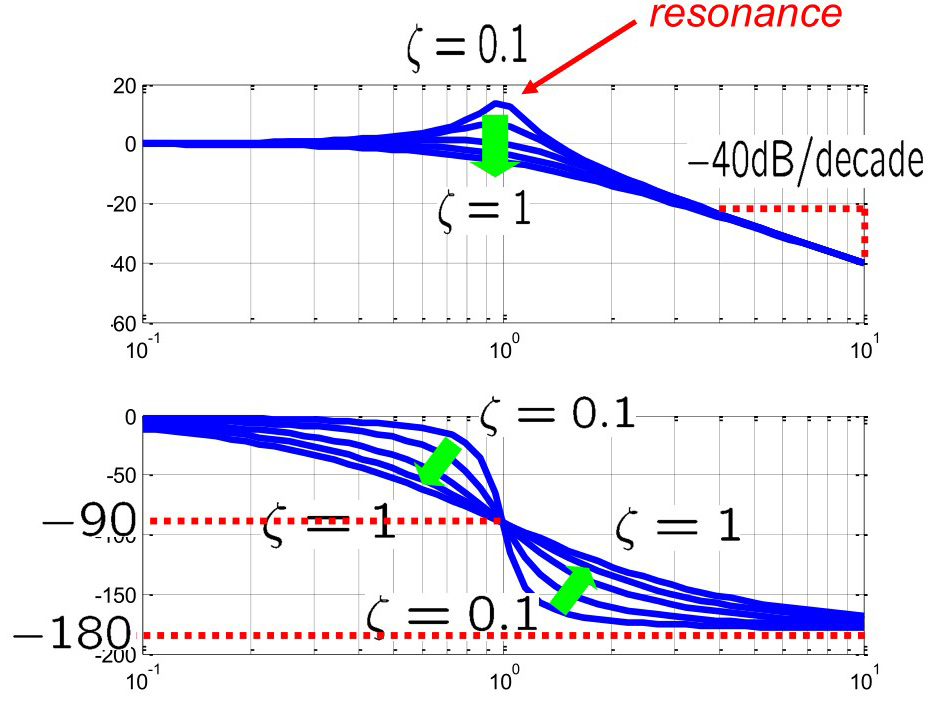
\includegraphics[width=\linewidth]{SecondOrderFreqResponse.jpg}
\end{Figure}
Resonant Frequency: $\omega_n \sqrt{1 - 2 \zeta^2} \approx \omega_n$

Peak Gain: \tab $\ds \frac{1}{2\zeta\sqrt{1-\zeta^2}} \approx \frac{1}{2\zeta}$

At the resonant frequency, the gain is unity when $\zeta = 1/\sqrt{2}$.

\subsection{Nyquist Stability}
For a open-loop transfer function $L(s)$:
\begin{itemize}
	\item CL system is stable $\iff Z := P + N = 0$
	\item $Z$: \# of CL poles in open RHP.
	\item $P$: \# of OL poles in open RHP.
	\item $N$: \# of clockwise encirclement of -1
	\item $N = -1$ is a counter-clockwise encirclement.
\end{itemize}

\subsection{Relative Stability}
Gain crossover frequency $\omega_g$:\\
\tab $\abs{L(j\omega_g)} = 1$

Phase crossover frequency $\omega_p$\\
\tab $\angle L(j\omega_p) = -180^\circ$

Gain Margin:\\
\tab $\ds \text{GM} = 20\log_{10}\frac{1}{\abs{L(j\omega_p)}}$

Phase Margin:\\
\tab $\ds \text{PM} = \angle L(j\omega_g) + 180^\circ$

% Footer content
\rule{0.3\linewidth}{0.25pt}
\scriptsize\\
Updated \today\\
\href{https://github.com/DonneyF/formula-sheets}{https://github.com/DonneyF/formula-sheets}

\end{multicols}
\end{document}
